\section{Computador} 
Construir um computador parece uma tarefa complicada e assustadora. Porem, uma CPU\footnote{CPU é a sigla para Central Process Unit, ou Unidade Central de Processamento. É o principal item de hardware do computador, que também é conhecido como processador, essa é a parte responsável por calcular e realizar tarefas determinadas pelo usuário.} é bastante simples em operação depois que os fundamentos por trás de todos os seus processos são compreendidos. Este cápitulo destina-se a executar o passo a passo para que qualquer pessoa interessada seja capaz em construir seu próprio computador e obter o conhecimento que acompanha o processo.
\subsection{Modulos}
Para facilitar o compreendimento, e também o desenvolvimento do computador, este capitulo será dividido em alguns subcapitulos, assim cada um abordará uma parte do computador. 
\subsubsection{Clock}
O clock do computador é uma parte essencial para o seu funcionamento. Este tem a função de sincronizar todas as operações. A ação mais rápida que o computador consegue executar é equivalente a uma vibração do seu clock.
\begin{figure}[h!] \centering 
  \makebox[\textwidth][c]{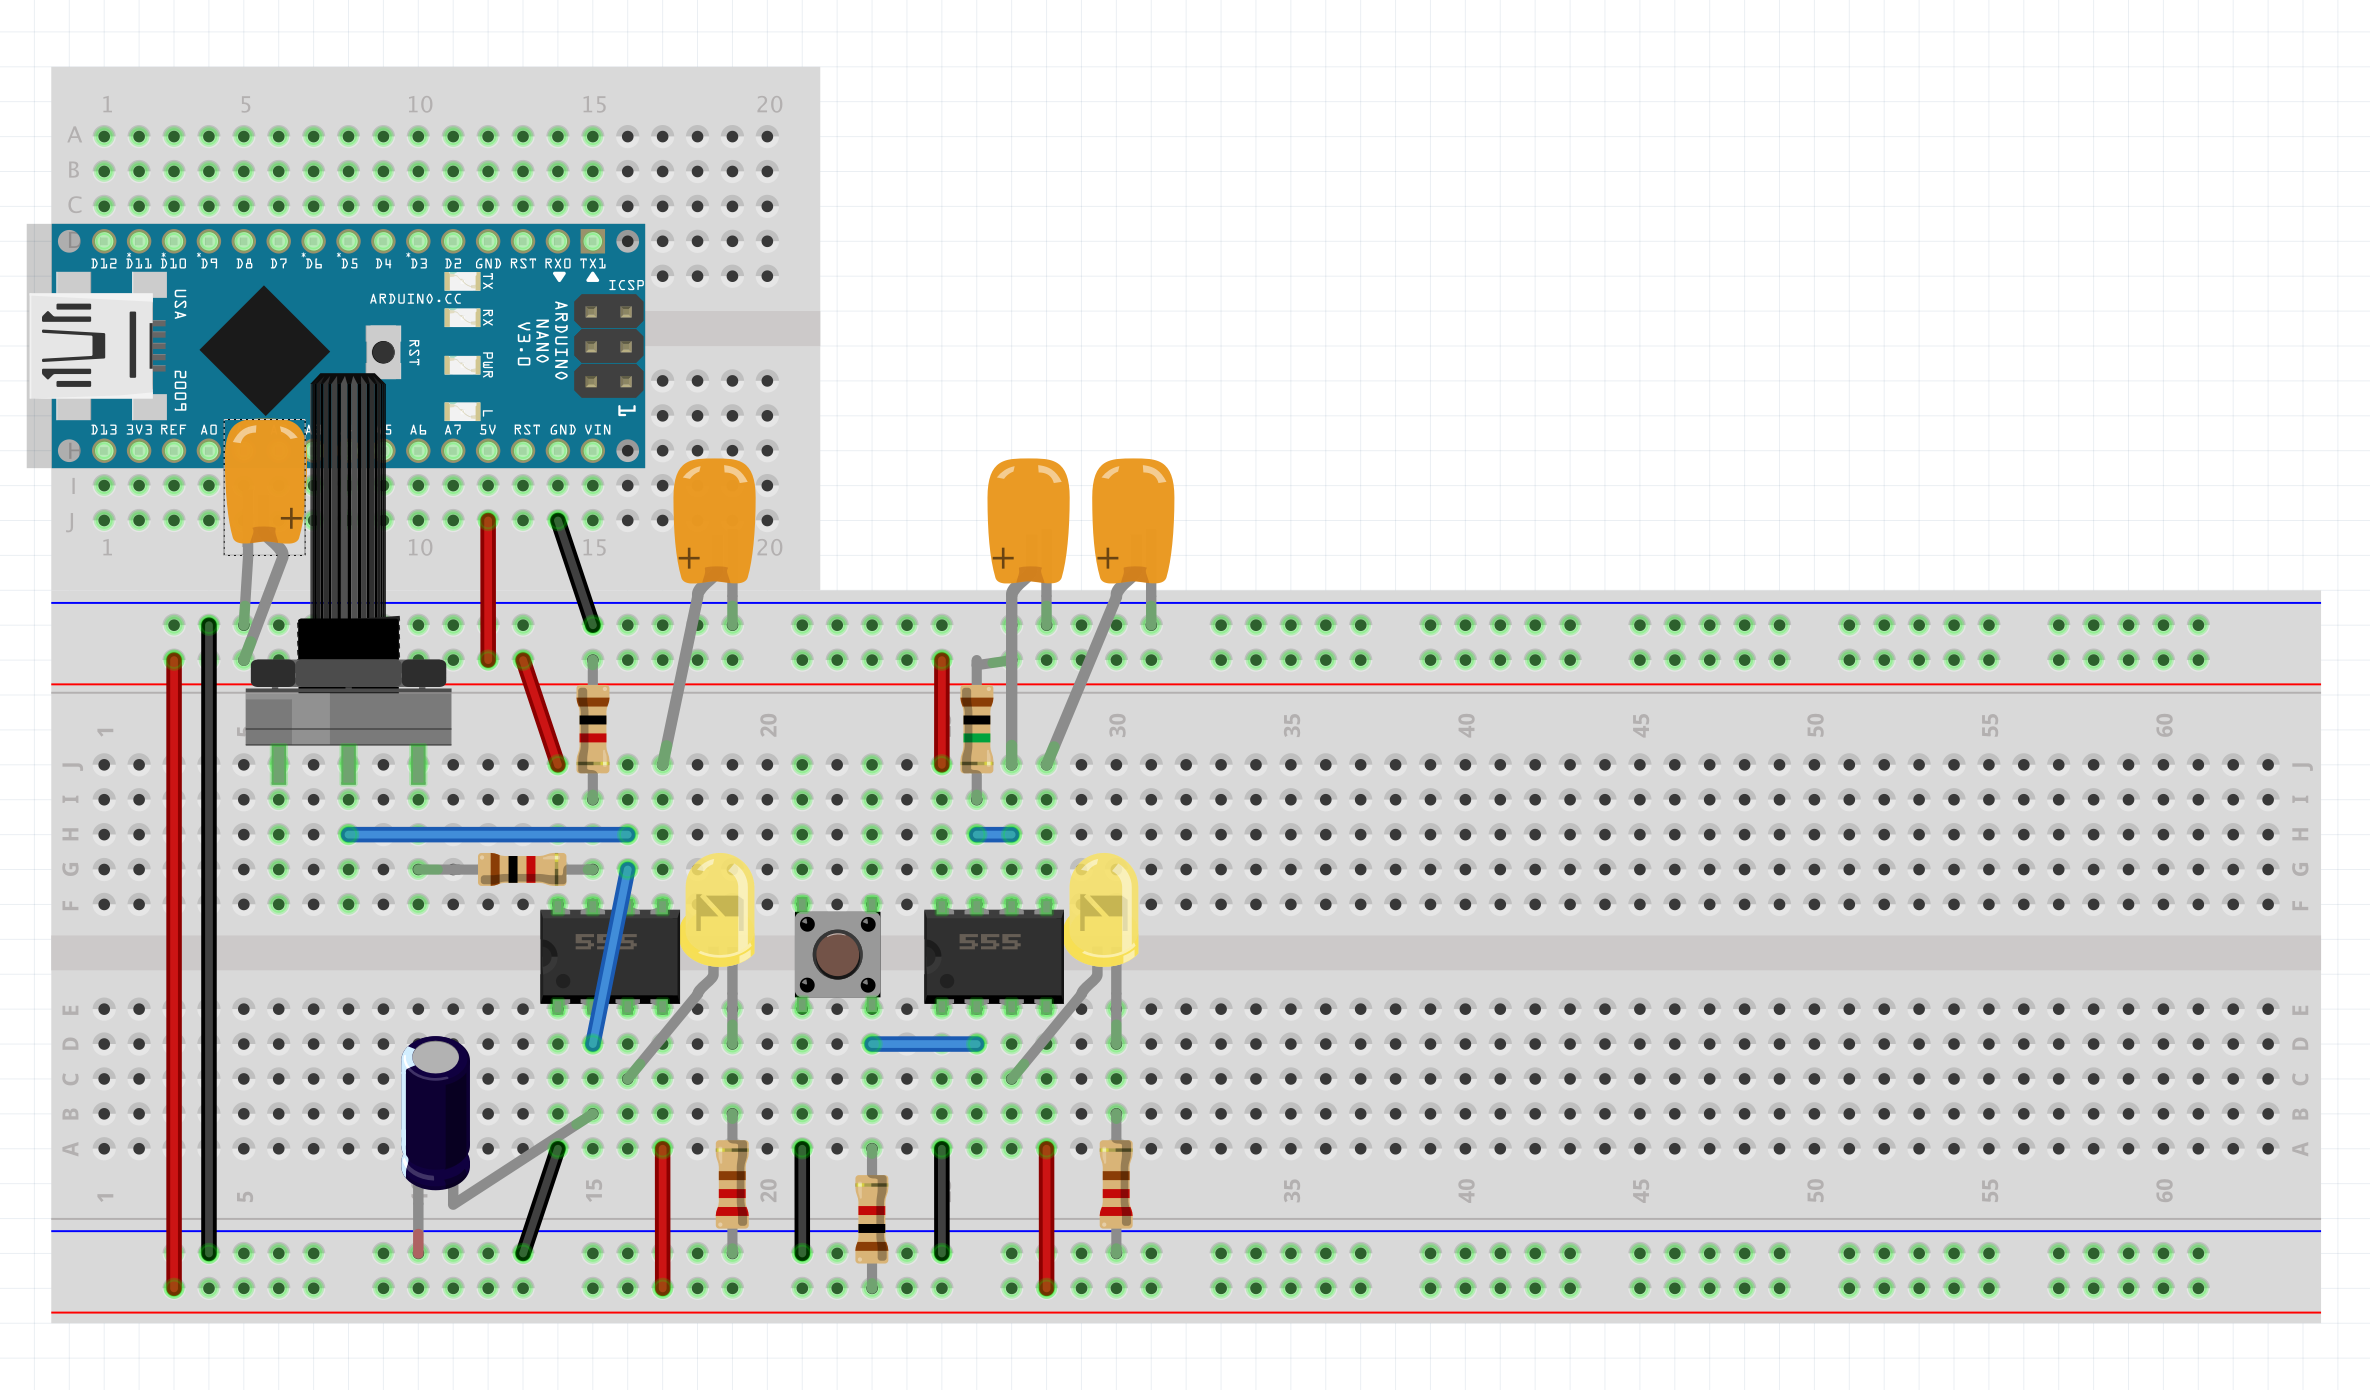
\includegraphics[width=0.8\textwidth]{clock}}
  \caption{\label{fig:1} Esquema do Clock} 
\end{figure}
\subsubsection{Materiais Necessários}
\newpage